\documentclass{article}
\usepackage{graphicx} % Required for inserting images
\usepackage{minted}

\title{Computational Geometry}
\author{Alex Zhou}
\date{April 2019}

\begin{document}

\maketitle

\section{Introduction}

In this project, we shall explore computational geometry on non-Euclidean spaces. In particular, we will focus on the extended complex plane model of spherical geometry and the disc model of hyperbolic geometry where we shall create some visualisations and examine the action of their isometry groups. Spherical, hyperbolic, together with Euclidean geometry form the three different verions of the parallel postulate and also the three different cases of Gaussian curvature. First, let us give a brief reminder of the definitions.

For spherical geometry, we work on the extended complex plane \(\hat{\mathbf{C}} = \mathbf{C} \cup \{\infty\}\) which has the topology of the one-point compactification of \(\mathbf{C}\). A spherical line in \(\mathbf{C} \cup \{\infty\}\) is either a straight line through the origin or a circle of the form
\[ \{ z \in \mathbf{C} : |z-a|^2 = |a|^2 + 1 \} \]
with \(a \in \mathbf{C}\). Under a stereographic projection, a spherical line corresponds to a great circle on the unit sphere embedded in \(\mathbf{R}^2\). Moreover, the stereographic projection preserves angles so it is conformal. A spherical triangle is formed by joining three points \(z_1, z_2, z_3 \in \hat{\mathbf{C}}\) by spherical lines. Given a spherical triangle with side lengths \(a,b,c\) and corresponding internal angles \(\alpha,\beta,\gamma\), the second law of cosines states
\[ \cos\alpha + \cos\beta\cos\gamma = \sin\beta\sin\gamma\cos\alpha. \]
The side lengths are measured using spherical distance.

For hyperbolic geometry, we shall take the Poincar\'{e} disc model \(D = \{z \in \mathbf{C} : |z| < 1\}\) with the induced topology from \(\mathbf{C}\). A hyperbolic line in \(D\) is either straight line through the origin or a circle of the form
\[ \{z \in \mathbf{C} : |z-a|^2  |a|^2 - 1\} \]
where \(|a| \in \mathbf{C} - \bar{D}\). Note that this differs from lines in the extended complex plane model of spherical geometry by a change of sign. A hyperbolic triangle is formed by joining three points \(z_1, z_2, z_3 \in D\) by hyperbolic lines. Given a hyperbolic triangle with side lengths \(a,b,c\) and corresponding internal angles \(\alpha,\beta,\gamma\), the second law of cosines states
\[ \cos\alpha + \cos\beta\cos\gamma = \sin\beta\sin\gamma\cosh\alpha. \]
The side lengths are measured using hyperbolic distance.

\section{Spherical Lines and Triangles}

Given two points \(z_1, z_2 \in \hat{\mathbf{C}}\), we aim to find the spherical line through \(z_1\) and \(z_2\). Let us first analyse the equation \(|z-a|^2 = |a|^2 + 1 \) by expanding the left hand side using \(|z|^2 = z\bar{z}\),
\[ |z-a|^2 = |z|^2 - z\bar{a} - \bar{z}a + |a|^2 \]
Equating to the right hand side and rearranging, we obtain
\[ |z|^2 - 1 = z\bar{a} + \bar{z}a, \]
which holds for \(z_1\) and \(z_2\). Setting \(b_1 = |z_1|^2 - 1\) and \(b_2 = |z_2|^2 - 1\) gives us a system of two linear equations
\begin{eqnarray*}
    z_1\bar{a} + \bar{z_1}a = b_1 \\
    z_2\bar{a} + \bar{z_2}a = b_2
\end{eqnarray*}
which by Cramer's rule has the following solution for \(a\),
\[ a = \frac{b_2 z_1 - b_1 z_2 }{z_1\bar{z_2} - \bar{z_1}z_2}. \]
Simplifying the denominator
\begin{eqnarray*}
    z_1\bar{z_2} - \bar{z_1}z_2 & = & z_1\bar{z_2} - \overline{z_1\bar{z_2}} \\
                                & = & 2i\Im(z_1\bar{z_2}). \\
\end{eqnarray*}
Substituting back for \(a\) gives the formula
\[ a = \frac{i}{2\det}(b_1z_2 - b_2z_1), \]
provided that \(\det = \Im(z_1\bar{z_2}) \neq 0\) which is the determinant of the matrix,
\[ \pmatrix{z_1 & \bar{z_1} \cr z_2 & \bar{z_2}}. \]
This is precisely the condition that \(z_1\) and \(z_2\) are not collinear with the origin: if we have \(z_1 = rz_2\) for some \(r \in \mathbf{R}-\{0\}\), then \(\frac{z_1}{z_2} \in \mathbf{R}\). Multiplying by \(|z_2|^2 \in \mathbf{R}\) gives \(z_1\bar{z_2} \in \mathbf{R}\) which is equivalent to \(\Im(z_1\bar{z_2)} = 0\). In this case, we take the straight line through \(z_1\) and \(z_2\) passing through the origin. The following is code of two functions in Python. The first takes two points and samples a user-defined number of points on the shortest arc of the spherical line between them. The second takes three points and uses the first function to define a spherical triangle. 


\begin{minted}[autogobble, linenos]{python}
    import numpy as np
    from matplotlib import pyplot as plt
    
    def spherical_line(z1, z2, n = 100):
        z1, z2 = complex(z1), complex(z2)
    
        # Identical points
        if np.isclose(z1, z2):
            return np.full(n, z1)
    
        # Colinearity with the origin
        det = np.imag((z1 * np.conj(z2)))
        if np.isclose(det, 0):
            return np.linspace(z1, z2, n, dtype = complex)
            
        # General case, circular arc
        b1, b2 = np.abs(z1)**2 - 1, np.abs(z2)**2 - 1
        centre = (1j / (2 * det)) * (b1 * z2 - b2 * z1)
        radius = np.sqrt(abs(centre)**2 + 1)
        theta1, theta2 = np.angle(z1 - centre), np.angle(z2 - centre)
        delta_theta = theta2 - theta1
    
        # Normalize angle difference to (-pi, pi]
        if delta_theta > np.pi:
            delta_theta -= 2 * np.pi
        elif delta_theta <= -np.pi: # Use <= to handle -pi case 
            delta_theta += 2 * np.pi
    
        # The adjusted end angle for linspace to trace the shorter arc
        theta_2 = theta1 + delta_theta
    
        # Generate points along the arc
        theta = np.linspace(theta1, theta_2, n)
        return centre + radius * np.exp(1j * theta)
    
    def spherical_triangle(z1, z2, z3, n = 100):
        arc = [
            spherical_line(z1, z2, n), 
            spherical_line(z2, z3, n), 
            spherical_line(z3, z1, n)
        ]
        triangle_path = np.concatenate(arc)
        return triangle_path
\end{minted}

Using this program, we can plot some examples of spherical triangles on the extended complex plane. Points collinear with the origin are joined using a straight line.

\begin{figure}
    \centering
    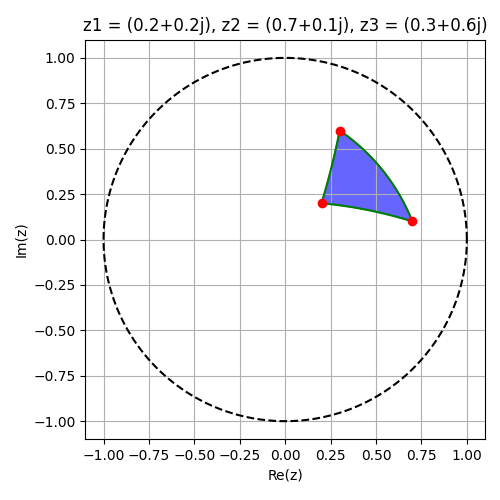
\includegraphics[width=0.495\linewidth]{images/sphere_circle_1.png}
        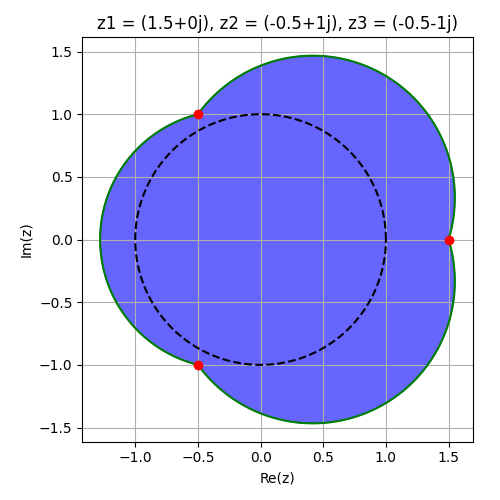
\includegraphics[width=0.495\linewidth]{images/sphere_circle_4.png}
    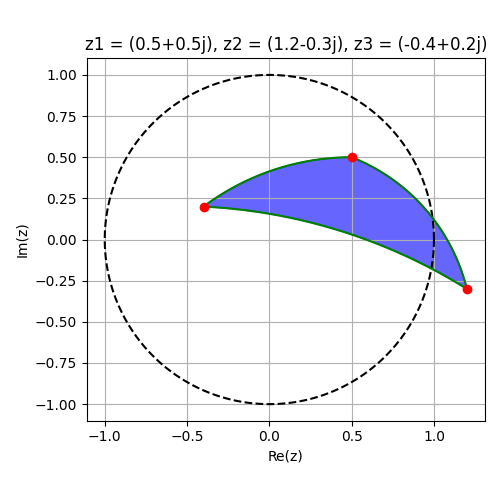
\includegraphics[width=0.495\linewidth]{images/sphere_circle_2.png}
    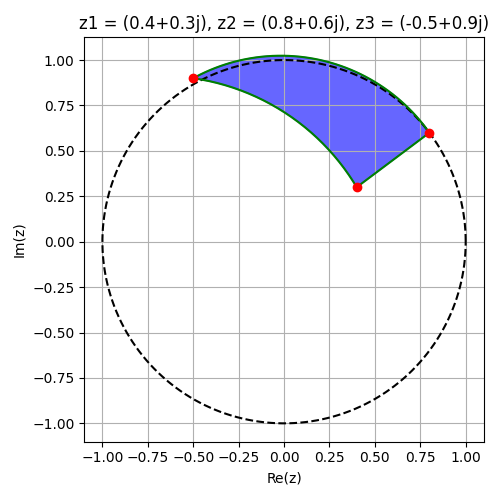
\includegraphics[width=0.495\linewidth]{images/sphere_circle_3.png}
    \caption{Examples of spherical triangles with the unit circle on the complex plane.}
    \label{fig:enter-label}
\end{figure}

Let \(z_0\) be an intersection point of a spherical line with the unit circle \(\{z \in \mathbf{C}:|z| = 1\}\). Then we claim that \(-z_0\) is also an intersection point. This is clear for lines passing through the origin. Otherwise, consider the equation with \(|z| = 1\)
\[ |z-a|^2 = |z+a|^2 = |z|^2 - z\bar{a} - \bar{z}a + a^2 = 1 - z\bar{a} - \bar{z}a + |a|^2, \]
and equating to \(|a|^2 + 1\) shows that
\[ z\bar{a} + \bar{z}a = 2\Re(z\bar{a}) = 0. \]
Solving this equation for a point that lies on the unit circle \(z = e^{i\theta}\), we obtain
\[ \Re(z\bar{a}) = \Re(e^{i\theta}|a|e^{-i\arg(a)}) = |a|\cos(\theta - \arg(a)), \]
which is zero when \(\theta = \arg(a) \pm \frac{\pi}{2}\) or when \(|a| = 0\) which are coinciding unit circles. Therefore, the intersection points lie on a diameter of the unit circle with angles orthogonal to angle of \(a\). 

To compute the angle of intersection \(\alpha\) at the intersection point \(z_0\) between the circles, we form the triangle with vertices \(0\), \(a\) and \(z_0\) with corresponding (opposite) side-lengths \(|z_0 - a| = \sqrt{|a|^2 + 1}\), \(|z_0| = 1\) and \(|a|\). The desired angle \(\alpha\) is the internal angle at the vertex \(z_0\). By the (normal) cosine law
\[ |a|^2 = 1 + |a|^2 + 1 - 2 \cos(\alpha)\sqrt{|a|^2 + 1} \]
which simplifies to
\[ \cos\alpha = \frac{1}{\sqrt{|a|^2 + 1}}. \]
If \(a = 0\), then the angle is \(0\) as the circles coincide. As \(|a| \to \infty\), the denominator gets larger, so the \(\cos(\alpha)\) gets closer to \(0\) and the angle tends to \(\frac{\pi}{2}\) (orthogonal). Indeed, we can see the limiting case as the situation where spherical line is a straight line through the origin.

\begin{figure}
    \centering
    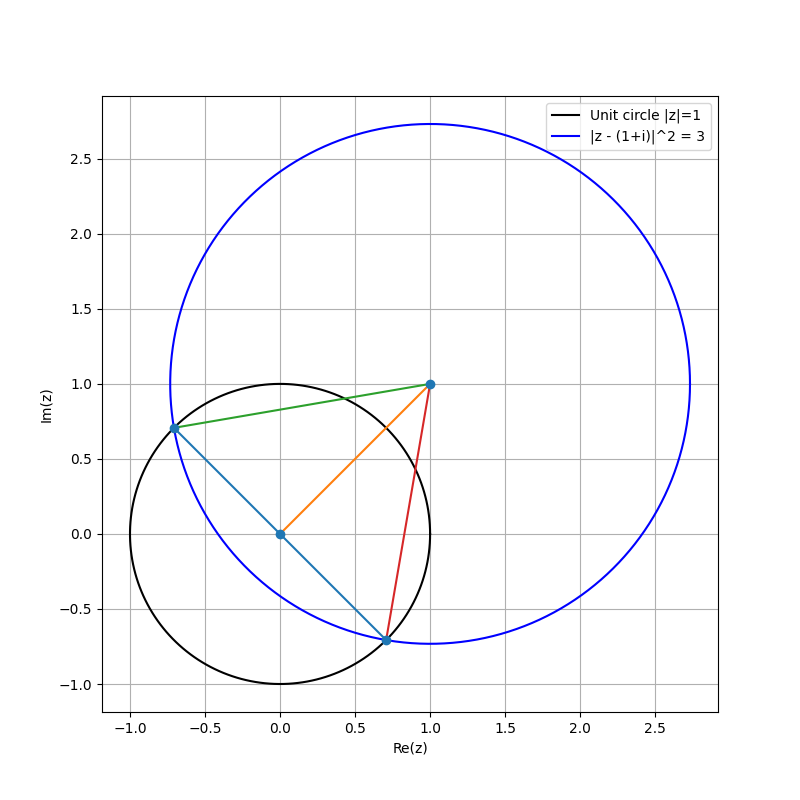
\includegraphics[width=1.0\linewidth]{images/sphere_intersect.png}
    \caption{Intersecting points are on a diameter of the unit circle and are orthogonal to \(a\).}
\end{figure}

We can also see this as a spherical triangle on the Riemann sphere and use the spherical law of cosines. Here, the unit circle maps by the stereographic projection (which preserves angles) to the equator, a spherical line is another (perhaps the same) great circle defined by the plane with normal vector \((\Re(a), \Im(a), 1)\); and the origin is the north pole. Consider the triangle formed by the north pole \(N = (0,0,1)\), the intersection point \(X_0\) and a 'pole' or highest point of the great circle 
\[ P = \frac{1}{\sqrt{|a|^2 + 1}}(-\Re(a), -\Im(a), 1 ). \]

The angle at the intersection point \(\phi\) is the angle between the equator and great circle; the (spherical) distance between \(X_0\) and \(P\) is \(\frac{\pi}{2}\); and the distance between \(P\) to \(N\) is the cosine of
\[ (0,0,1) \cdot \frac{1}{\sqrt{|a|^2 + 1}} (-\Re(a), -\Im(a), 1) = \frac{1}{\sqrt{|a|^2+1}};\]
and the distance between \(N\) and \(X_0\) is \(\frac{\pi}{2}\)
Applying the spherical cosine law gives
\[ \frac{1}{\sqrt{|a|^2+1}} + \cos\frac{\pi}{2}\cos\frac{\pi}{2}= \sin\frac{\pi}{2}\sin\frac{\pi}{2}\cos\phi, \]
yielding the exact same formula
\[ \cos\phi = \frac{1}{\sqrt{|a|^2 + 1}} \]
as desired.

\section{Hyperbolic Lines and Triangles}
Turning our attention now to the hyperbolic case, let \(z_1, z_2 \in D\) be two points and let us now analyse the hyperbolic line equation \(|z-a|^2 = |a|^2 - 1\) using the same expansion
\[ |z-a|^2 = |z|^2 - z\bar{a} - \bar{z}a + |a|^2, \]
which now yields
\[ |z|^2 + 1 = z\bar{a} + \bar{z}a, \]
which holds for \(z_1\) and \(z_2\). Repeating our previous methods, set \(b_1 = |z_1|^2 + 1\) and \(b_2 = |z_2|^2 + 1\) to obtain two linear equations
\begin{eqnarray*}
    z_1\bar{a} + \bar{z_1}a = b_1 \\
    z_2\bar{a} + \bar{z_2}a = b_2
\end{eqnarray*}
which by Cramer's rule has the following solution for \(a\),
\[ a = \frac{b_2z_1 - b_1z_2}{z_1\bar{z_2} - \bar{z_1}z_2}. \]
Again the denominator is given by
\[ z_1\bar{z_2} - \bar{z_1}z_2 = 2i\Im(z_1\bar{z_2}), \]
so
\[ a = \frac{i}{2\det}(b_1z_2 - b_2z_1), \]
provided \(\det = \Im(z_1\bar{z_2}) \neq 0\), which is the determinant of the matrix
\[ \pmatrix{z_1 & \bar{z_1} \cr z_2 & \bar{z_2}}, \]
which analogously means \(z_1\) and \(z_2\) are not collinear with the origin. The following is the hyperbolic version of our previous code:

\begin{minted}[autogobble, linenos]{python}
    def hyperbolic_line(z1, z2, n = 100):
        z1 = complex(z1)
        z2 = complex(z2)
    
        # Identical points
        if np.isclose(z1, z2):
            return np.full(n, z1)
    
        # Colinearity with the origin
        det = np.imag((z1 * np.conj(z2)))
        if np.isclose(det, 0):
            return np.linspace(z1, z2, n, dtype = complex)
            
        # General case, circular arc
        A1, A2 = np.abs(z1)**2 + 1, np.abs(z2)**2 + 1
        centre = (1j / (2 * det)) * (A1 * z2 - A2 * z1)
        radius = np.sqrt(abs(centre)**2 - 1)
        theta1, theta2 = np.angle(z1 - centre), np.angle(z2 - centre)
        delta_theta = theta2 - theta1
    
        # Normalize angle difference to (-pi, pi]
        if delta_theta > np.pi:
            delta_theta -= 2 * np.pi
        elif delta_theta <= -np.pi: # Use <= to handle -pi case 
            delta_theta += 2 * np.pi
    
        # The adjusted end angle for linspace to trace the shorter arc
        theta_2 = theta1 + delta_theta
    
        # Generate points along the arc
        theta = np.linspace(theta1, theta_2, n)
        return centre + radius * np.exp(1j * theta)

    def hyperbolic_triangle(z1, z2, z3, n = 100):
        arc = [
            hyperbolic_line(z1, z2, n), 
            hyperbolic_line(z2, z3, n), 
            hyperbolic_line(z3, z1, n)
        ]
        triangle_path = np.concatenate(arc)
        return triangle_path
\end{minted}

We also plot some examples of hyperbolic triangles on the complex plane, superimposed with the unit circle. 

\begin{figure}
    \centering
    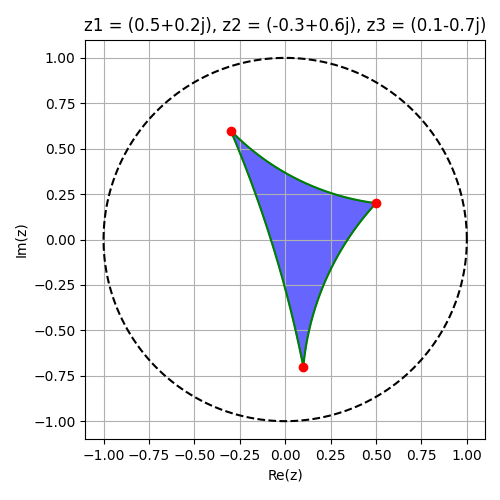
\includegraphics[width=0.495\linewidth]{images/hyperbolic_circle_1.png}
    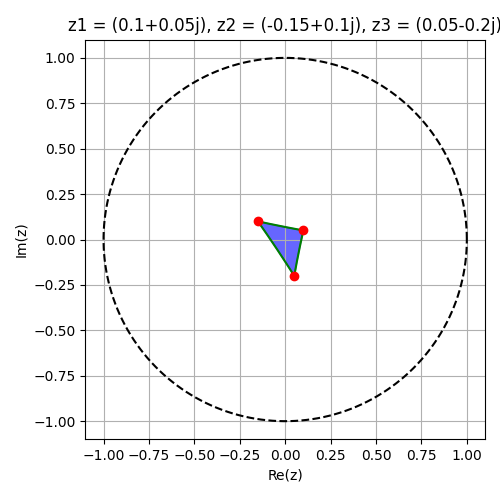
\includegraphics[width=0.495\linewidth]{images/hyperbolic_circle_2.png}
    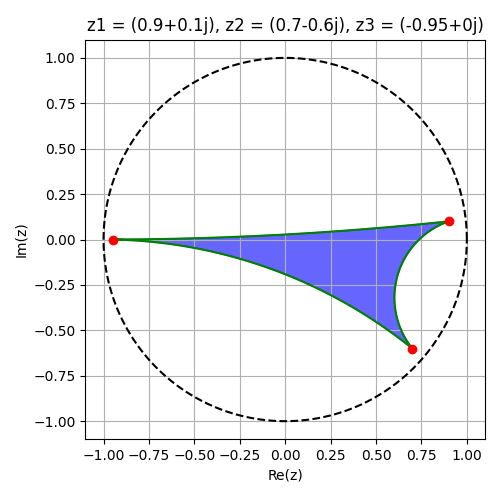
\includegraphics[width=0.495\linewidth]{images/hyperbolic_circle_3.png}
    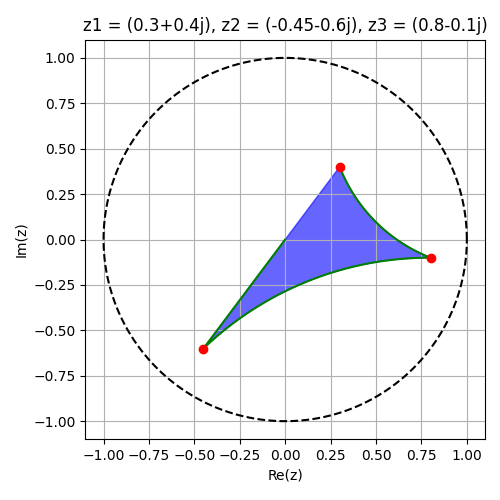
\includegraphics[width=0.495\linewidth]{images/hyperbolic_circle_4.png}
    \caption{Examples of hyperbolic triangles with the unit circle on the complex plane.}
\end{figure}

Let \(z_0 = e^{i\theta}\) be an intersection point of a hyperbolic line with the unit circle \(\{z \in \mathbf{C}:|z| = 1\}\). The same analysis as before shows
\[ |z-a|^2 = |z|^2 - z\bar{a} - \bar{z}a + |a|^2 = 1 - z\bar{a} - \bar{z}a + |a|^2, \]
where equating to \(|a|^2 - 1\) now yields
\[ \frac{1}{2}(z\bar{a} + \bar{z}a) = \Re(z\bar{a}) = 1. \]
Solving this equation for \(z = e^{i\theta}\),
\[ \Re(e^{i\theta}|a|e^{-i\arg(a)}) = |a|\cos(\theta - \arg(a)) = 1, \]
which gives
\[ \cos(\theta - \arg(a)) = \frac{1}{|a|}. \]
yielding the solutions \(\theta = \arg(a) \pm \arccos(1/|a|)\). For this to be valid, we require \(|a| > 1\) which is required for a non-negative radius of our circle. The case where \(|a| = 1\) describes a single point since the unit circle describes a 'boundary at infinity'. In the straight line through the origin case, where the intersection points form a diameter.

The angle of intersection \(\alpha\) turns out to be quite interesting in the hyperbolic situation. Once again, let us form a hyperbolic triangle with vertices at \(0\), \(a\) and the intersection point \(z_0\). The corresponding (opposite) sides-lengths are then \(\sqrt{|a|^2 - 1}\), \(|z_0| = 1\) and \(|a|\). The desired angle is the internal angle at \(z_0\) which by the (normal) cosine law can be computed as
\[ |a|^2 = 1 + |a|^2 - 1 - 2\cos(\alpha)\sqrt{|a|^2 - 1} \]
which results in
\[ \cos\alpha = 0. \]
This means that hyperbolic lines intersect orthogonally with the unit circle. Taking \(|a| \to \infty\) is once again the situation where the hyperbolic line is a straight line through the origin, which certainly orthogonally intersects the unit circle.

\begin{figure}
    \centering
    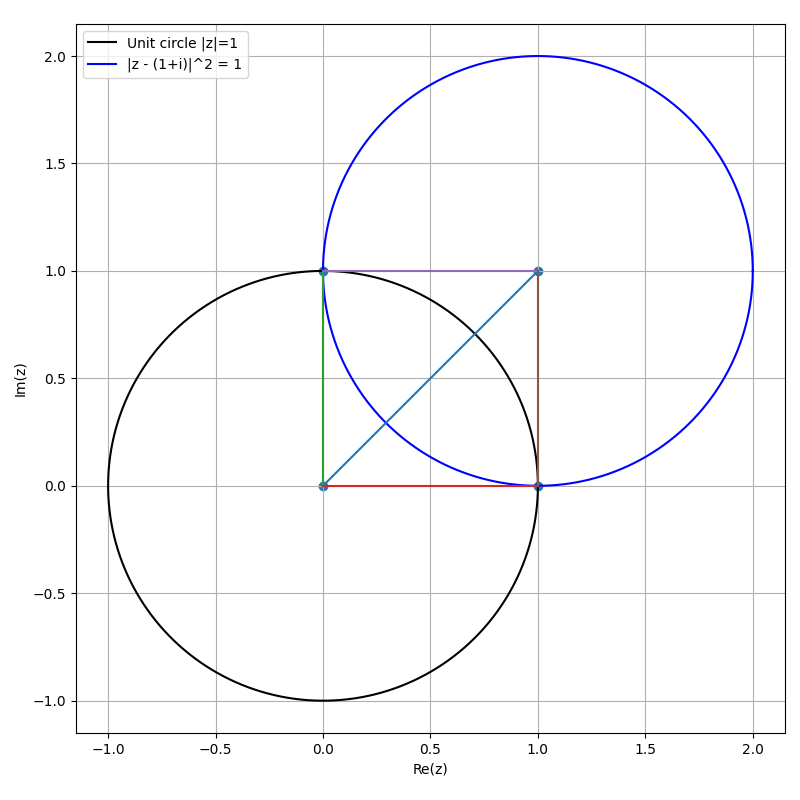
\includegraphics[width=1.0\linewidth]{images/hyperbolic_intersect.png}
    \caption{Intersecting points on a hyperbolic line.}
\end{figure}

This fact can also be proved using the hyperbolic cosine law which we shall omit.

\section{Regular Polygons}

A spherical or hyperbolic \(n\)-gon is obtained by joining \(n\) vertices by spherical or hyperbolic lines. 

Consider the roots of \(z^n =  r^n\) which form a spherical or hyperbolic \(n\)-gon. The vertices are given by \(z_k = re^{i\theta_k}\), where \(\theta_k = \frac{2k\pi}{n}\) for \(k = 0, \dots, n-1\). Let \(\phi = \frac{2\pi}{3}\) be the internal angle at the vertex \(z_0 = r\). By rotational symmetry, this internal angle is the same at all vertices.

Divide the \(n\)-gon into \(n\) congruent isosceles triangles with a common vertex at the origin. Consider a particular triangle \((T\) formed by vertices \(0\), \(z_k\) and \(z_{k+1}\). Then the angles at each vertex are \(\frac{2\pi}{n}\), \(\frac{\phi}{2} = \frac{\pi}{3}\) and \(\frac{\phi}{2} = \frac{\pi}{3}\) respectively. 

In the spherical case, by the angular defect formula, the sum of the angles must be greater than \(\pi\), hence
\[ \frac{2\pi}{n} + \frac{\pi}{3} + \frac{\pi}{3} > \pi \quad \Rightarrow \quad \frac{2}{n} + \frac{2}{3} > 1, \]
which implies \(n < 6\). The area of this triangle is then
\[ \frac{2\pi}{n} + \frac{\pi}{3} + \frac{\pi}{3} - \pi = \frac{2\pi}{n} - \frac{\pi}{3}, \]
so the area of the polygon is
\[ n\left(\frac{2\pi}{n} - \frac{\pi}{3}\right) = 2\pi - \frac{n\pi}{3}. \]

Similarly, for the hyperbolic case, the sum of the angles must be less than \(\pi\), which using the dual angular defect formula implies \(n > 6\) with the area of the triangle being
\[ \pi - \left(\frac{2\pi}{n} + \frac{\pi}{3} + \frac{\pi}{3}\right) = \frac{\pi}{3} - \frac{2\pi}{n},\]
which yields the area of the polygon
\[ n\left(\frac{\pi}{3} - \frac{2\pi}{n}\right) = \frac{n\pi}{3} - 2\pi. \]

Let us now consider subdividing the \(n\)-gons into \(2n\) triangles with internal angles \(\frac{\pi}{2}, \frac{\pi}{3}, \frac{\pi}{n}\), also known as the \((2, 3, n)\) Schwarz triangles. Let \(m_k\) be the (spherical/hyperbolic) midpoint of the side between vertices \(z_k\) and \(z_{k+1}\). Form the triangle with vertices \(0\), \(z_k\) and \(m_k\) with the respective angles \(\frac{\pi}{n}, \frac{\pi}{3}, \frac{\pi}{2}\). We shall use the second law of cosines to relate the lengths of the triangle to the angles. 

In the spherical case, let \(\rho_z\) be the spherical distance between the origin to a vertex and \(\rho_m\) be the spherical distance between the origin to a midpoint. Then
\[ \cos\frac{\pi}{2} + \cos\frac{\pi}{n}\cos\frac{\pi}{3} = \sin\frac{\pi}{n}\sin\frac{\pi}{3}\cos\rho_z, \]
where rearranging gives
\[ \cos\rho_z = \frac{\cot\frac{\pi}{n}}{\sqrt{3}}, \]
which confirms \(n < 6\) since we require \(\cot\frac{\pi}{n} < \sqrt{3}\). Also
\[ \cos\frac{\pi}{3} + \cos\frac{\pi}{n}\cos\frac{\pi}{2} = \sin\frac{\pi}{n}\sin\frac{\pi}{2}\cos\rho_m \]
rearranges to
\[ \cos\rho_m = \frac{1}{2\sin\frac{\pi}{n}}, \]
which similarly confirms \(n < 6\) via \(\sin\frac{\pi}{n} > \frac{1}{2}\). 

Recall that the spherical distance between \(0\) and \(z\) is \(2\arctan|z|\). Together with a standard trigonometric identity 
\(\cos(t) = \frac{1 - \tan^2(t/2)}{1 + \tan^2(t/2)}, \)
the cosine of the spherical distance from \(0\) to \(z_k\) satisfies
\[ \cos\rho_z = \frac{1-r^2}{1+r^2}, \]
hence
\[ |z_k|^2 = r^2 = \frac{1 - \cos\rho_z}{1 + \cos\rho_z} = \frac{1 - \frac{1}{\sqrt{3}}\cot\frac{\pi}{n}}{1 + \frac{1}{\sqrt{3}}\cot\frac{\pi}{n}} = \frac{\sqrt{3} - \cot\frac{\pi}{n}}{\sqrt{3} + \cot\frac{\pi}{n}}. \]
This determines the radius \(r\) for valid \(n < 6\) and we already know the angle is \(\theta_k = \frac{2k\pi}{n}\). We perform the same calculation to obtain
\[ |m_k|^2 = \frac{1 - \cos\rho_m}{1 + \cos\rho_m} = \frac{1 - \frac{1}{2\sin\frac{\pi}{n}}}{1 + \frac{1}{2\sin\frac{\pi}{n}}} = \frac{2\sin\frac{\pi}{n} - 1}{2\sin\frac{\pi}{n} + 1}. \]
The midpoint \(m_k\) lies halfway between vertices \(z_k\) and \(z_{k+1}\) in terms of angle from the origin, thus the angle is the following average
\[ \frac{1}{2} \left(\frac{2k\pi}{n} + \frac{2(k+1)\pi}{n}\right) = \frac{(2k+1)\pi}{n}. \]

Without fully going into all the details, for the hyperbolic case, we swap the cosine of spherical distances with the hyperbolic cosine of hyperbolic distances. This means that
\[ \cosh\rho_z = \frac{\cot\frac{\pi}{n}}{\sqrt{3}}, \]
and 
\[ \cosh\rho_m = \frac{1}{2\sin\frac{\pi}{n}}, \]
which is now valid for when \(\cosh\rho_z > 1\) which means \(n > 6\). Using the hyperbolic identity \(\cosh(t) = \frac{1+\tanh^2(t/2)}{1-\tanh^2(t/2)}\), we again find
\[ |z_k|^2 = r^2 = \frac{\cosh\rho_z - 1}{\cosh\rho_z + 1} = \frac{\frac{1}{\sqrt{3}}\cot\frac{\pi}{n} - 1}{\frac{1}{\sqrt{3}}\cot\frac{\pi}{n} + 1} = \frac{\cot\frac{\pi}{n} - \sqrt{3}}{\cot\frac{\pi}{n} + \sqrt{3}}, \]
with known angle \(\theta_k = \frac{2k\pi}{n}\). For the midpoints, we have
\[ |m_k|^2 = \frac{\cosh\rho_m - 1}{\cosh\rho_m + 1} = \frac{\frac{1}{2\sin\frac{\pi}{n}} - 1}{\frac{1}{2\sin\frac{\pi}{n}} + 1} = \frac{1 - 2\sin\frac{\pi}{n}}{1 + 2\sin\frac{\pi}{n}}, \]
with angles 
\[ \frac{(2k + 1)\pi}{n}. \]
We plot the cases using our spherical and hyperbolic line functions for the cases \(5\) and \(7\) below.

\begin{figure}
    \centering
    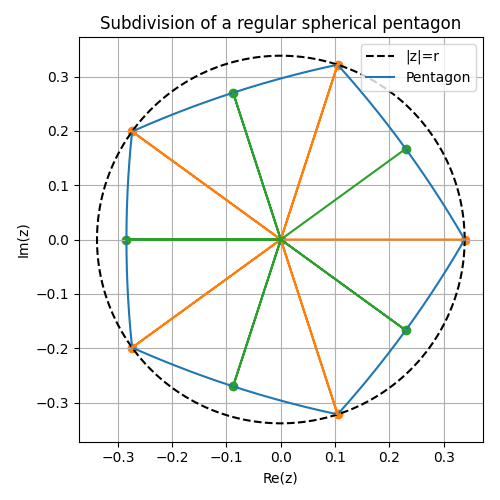
\includegraphics[width=0.495\linewidth]{images/sphere_reg.png}
    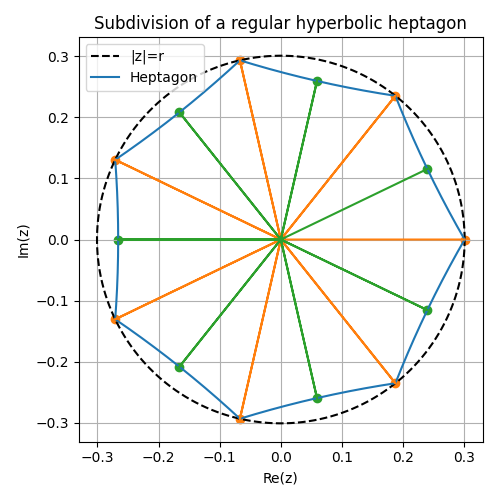
\includegraphics[width=0.495\linewidth]{images/hyperbolic_reg.png}
    \caption{Subdivision of a regular \(n\)-gon with internal angles \(\frac{2\pi}{3}\).}
\end{figure}

\section{Symmetry Groups}

Let \(p > 2\) be a prime number. Let \(\mathrm{SL}((2,p)\) be the finite group of \(2 \times 2\) matrices with entries in \(\mathbf{Z}/p\mathbf{Z}\) and with determinant \(1\). Let \(\mathrm{PSL}(2, P)\) be the quotient of \(\mathrm{SL}((2,p)\) by the subgroup \(\{\pm I\}\) of order \(2\). It can be shown that \(\mathrm{PSL}((2,p)\) is generated by
\[ \sigma_1 = \pm \pmatrix{0 & 1 \cr -1 & 0}, \quad \sigma_2 = \pm \pmatrix{0 & -1 \cr 1 & -1}, \quad \sigma_3 = \pm \pmatrix{1 & 1 \cr 0 & 1}.   \]
An inversion in a Euclidean circle \(C\) is a map of the form
\[ z \mapsto \frac{a\bar{z}+b}{c\bar{z} + d} \]
that fixes every point of \(C\). For example, inversion in the unit circle is \(z \mapsto \frac{1}{\bar{z}}\). Let \(L\) be a spherical or hyperbolic line. A reflection in \(L\) is defined to be either a Euclidean reflection if \(L\) is a straight line or an inversion if \(L\) is a circle.

Now consider a triangle \(\Delta_0\) from before which form a subdivision of a regular \(n\)-gon with internal angle \(\frac{2\pi}{3}\) where \(n = p\) is now prime. Let \(R_1\), \(R_2\) and \(R_3\) be reflections in the sides \(L_1\), \(L_2\) and \(L_3\) of \(\Delta_0\) opposite the vertices \(V_1\), \(V_2\) and \(V_3\) with the respective internal angles \(\frac{\pi}{2}, \frac{\pi}{3}, \frac{\pi}{p}\). 

We aim to describe the compositions of these reflections
\[ S_1 = R_2R_3, \quad S_2 = R_3R_1, \quad S_3 = R_1,R_2. \].
Without loss of generality, take \(V_1 = m_0\), \(V_2 = z_0 = r\) and \(V_3 = 0\). 
\begin{enumerate}
    \item \(L_1\) is a straight line through the origin on the real axis, so a reflection \(R_1\) corresponds to conjugation \(z \mapsto \bar{z}\). 

    \item \(L_2\) is a straight line through the origin with angle \(\frac{\pi}{p}\) so the reflection \(R_2\) is given by\(z \mapsto \bar{z}e^{2\pi i/p}\). 
    
    \item \(L_3\) is an arc of a Euclidean circle \(|z-a|^2 = R^2\). The reflection \(R_3\) is given by an inversion of this circle
    \[ z \mapsto a + \frac{R^2}{\bar{z} - \bar{a}} = \frac{a\bar{z} + (R^2 - |a|^2)}{\bar{z} - \bar{a}} = \frac{a\bar{z} \pm 1 }{\bar{z} - \bar{a}}, \]
    where \(a\) is given by a formula we calculated in the previous sections.
    \[ a = \frac{i}{-2|z_0||m_0|\sin\frac{\pi}{p}} ((|z_0|^2 \mp 1)m_0 - (|m_0|^2 \mp 1)z_0). \]
\end{enumerate}

We can now compute the compositions of these reflections. These are rotations, since the composition of two orientation-reversing transformations gives a orientation-preserving transformation. Since angles are preserved under the stereographic projection, we can see that the angle of rotation of two reflections is twice the angle of the intersection of the axes of reflection about the point of intersection.

\begin{enumerate}
    \item \(S_1\) is a rotation by angle \(\pi\) at \(m_0\) which has order \(2\),
    \[S_1z = R_2R_3z = R_2\frac{a\bar{z} \pm 1 }{\bar{z}} = e^{\frac{2\pi i}{p}} \left(\frac{\bar{a}z \pm 1}{z - a}\right). \] 
    \item \(S_2\) is a rotation by angle \(-\frac{2\pi}{3}\) at \(z_0\) which has order \(3\), 
    \[S_2z = R_3R_1z = R_3\bar{z} = \frac{az \pm 1}{z - \bar{a}}. \]
    \item \(S_3\) is a rotation by angle \(-\frac{2\pi}{p}\) at the origin which has order \(p\),
    \[S_3z = R_1R_2z = R_1\bar{z}e^{2\pi i/p} = ze^{-2\pi i/p}.\] 
\end{enumerate}

It turns out that the orders of these compositions match the order of the generators of \(\mathrm{PSL}(2, p)\).

\begin{enumerate}
    \item Clearly
    \[\sigma_1^2 = \pmatrix{0 & 1 \cr -1 & 0}\pmatrix{0 & 1 \cr -1 & 0} = \pmatrix{-1 & 0 \cr 0 & -1} = -I, \]
    
    \item and also
    \[ \sigma_2^3 = \pm\pmatrix{0 & -1 \cr 1 & -1} \pmatrix{0 & -1 \cr 1 & -1} \pmatrix{0 & -1 \cr 1 & -1} = \pmatrix{1 & 0 \cr 0 & 1} = I. \]
    \item By induction,
    \[\sigma_3^k = (-1)^{k \bmod 2} \pmatrix{1 & k \cr 0 & 1} \]
    which is equal \(\pm I\) if and only if \(k = p\). Notice that here we require \(p \neq 2\) and \(p\) is prime so has no non-trivial factors.
\end{enumerate}

We encode all these reflections for both the spherical and hyperbolic cases in the following code:

\begin{minted}[autogobble, linenos]{python}
    def fundamental_triangle(n):
        cot = 1 / np.tan(np.pi / n)
        sin = np.sin(np.pi / n)
        sqrt3 = np.sqrt(3)
        sign = 1 if n < 6 else -1
        vertex_radius = np.sqrt( sign*(sqrt3 - cot) / (sqrt3 + cot) )
        vertex = vertex_radius + 0j
        midpoint_radius = np.sqrt( sign*(2*sin - 1) / (2*sin + 1) )
        midpoint = midpoint_radius * np.exp(1j*np.pi/n)
        return midpoint, vertex, 0
        
    def R1(z, n):
        return np.conj(z)
    def R2(z, n):
        return np.conj(z) * np.exp(2j*np.pi / n)
    def R3(z, n):
        z1, z2 = fundamental_triangle(n)[0:2]
        det = np.imag((z1 * np.conj(z2)))
        sign = 1 if n < 6 else -1
        b1, b2 = np.abs(z1)**2 - sign, np.abs(z2)**2 - sign
        centre = (1j / (2 * det)) * (b1 * z2 - b2 * z1)
        return (centre * np.conj(z) + sign) / (np.conj(z) - np.conj(centre))
        
    def S1(z, n):
        return R2(R3(z, n), n)
    def S2(z, n):
        return R3(R1(z, n), n)
    def S3(z, n):
        return R1(R2(z, n), n)
\end{minted}

\section{Tessellations}

Let \(g \in \mathrm{PSL}(2, p)\) and let \(\Delta\) be a triangle. The pair \((g, \delta)\) is called admissible if it is obtained from \((\pm I, \Delta_0)\) by a sequence of operations replacing \((g, \Delta)\) with \((\sigma_i g, S_i\Delta)\) for some \(i = 1,2,3\). We can list all the elements of \(\mathrm{PSL}(2, p)\) by repeatedly multiplying \(\pm I\) with the generators \(\sigma_i\) until no new elements are found. The following program uses a breadth first search (BFS) algorithm to repeatedly multiply products of given cyclic generators to find all the elements of the projective special linear finite group.

\begin{minted}[autogobble, linenos]{python}
    import numpy as np
    from collections import deque
    
    def canonical_rep(mat, p):
        # Quotient by +/= I
        mat_mod = np.mod(mat, p)
        neg_mod = np.mod(-mat, p)
        return min(mat_mod.tobytes(), neg_mod.tobytes())
    
    def list_of_words(generators, p):
        queue = deque()
        seen = dict()
        
        # Set identity
        identity = np.identity(2, dtype=int)
        seen[canonical_rep(identity, p)] = []
        queue.append((identity, []))
    
        while queue:
            mat, word = queue.popleft()
            for name, gen in generators:
                new_mat = np.mod(mat @ gen, p)
                key = canonical_rep(new_mat, p)
                if key not in seen:
                    new_word = word + [name]
                    seen[key] = new_word
                    queue.append((new_mat, new_word))
    
        # Output words (can also modify to print matrices)
        #return [(np.frombuffer(k, dtype=int).reshape(2,2), w) for k, w in seen.items()]
        return [w for k, w in seen.items()]
\end{minted}

Let \(g \in \mathrm{PSL}(2,p)\). We want to find a triangle \(\Delta\) such that \((g,\Delta)\) is admissible. This can be found by generating \(g\) as a product of the generators \(\sigma_i\), then composing corresponding transformations \(S_i\) and finally applying this composition to the fundamental triangle \(\Delta_0\). We use the following function which takes a triangle defined by three vertices in \(\mathbf{C}\) and an element \(g \in \mathrm{PSL}(2, p)\) expressed as a word of right multiplication by the generating matrices \(\sigma_i\). It then left composes the vertices with the corresponding transformations \(S_i\) to obtain a new triangle.

\begin{minted}[autogobble, linenos]{python}
    def transform_point(group_element, v1, v2, v3)
        for i in range(len(group_element) - 1, -1, -1):
            match element[i]:
                case 1:
                    w1, w2, w3 = S1(w1, n), S1(w2, n), S1(w3, n)
                case 2:
                    w1, w2, w3 = S2(w1, n), S2(w2, n), S2(w3, n)
                case 3:
                    w1, w2, w3 = S3(w1, n), S3(w2, n), S3(w3, n)
        return [w1, w2, w3]
\end{minted}

Recall that the order of \(\mathrm{GL}(2,p)\) is \((p^2 - 1)(p^2 - p)\) as there are \(p^2 - 1\) choices for the first column excluding the zero vector and \(p^2 - p\) choices for the second vector excluding multiples of the first vector. The determinant map 
\[ \det: \mathrm{GL}(2,p) \to (\mathbf{Z}/\mathbf{Z}p)^\times \]
is a homomorphism with kernel \(\mathrm{SL}(2,p)\) (the matrices with determinant \(1\)) which has order \(p-1\), so the first isomorphism theorem of groups gives that the order of \(\mathrm{SL}(2,p)\) is 
\[ \frac{(p^2 - 1)(p^2-p)}{p-1}  = p(p^2-1). \]
Since \(\mathrm{PSL}(p,2)\) is a quotient of \(\mathrm{SL}(2,p)\) by a group of order \(2\), then its order must be equal to \(\frac{1}{2} p(p^2-1)\). The number of admissible triangles we can expect to find is equal to the order of \(\mathrm{PSL}(2,p)\).

Generating the admissible triangles in this way, we can expect there to be no more triangles. Let \(T\) be the complete set of all such triangles. Applying a transformation \(S_i\) to a triangle \(\Delta_g \in T\) generated by \(S_g\) yields \(S_iS_g\Delta_0\), where the composite \(S_iS_g\) corresponds to the group element \(\sigma_ig\).

\begin{figure}
    \centering
    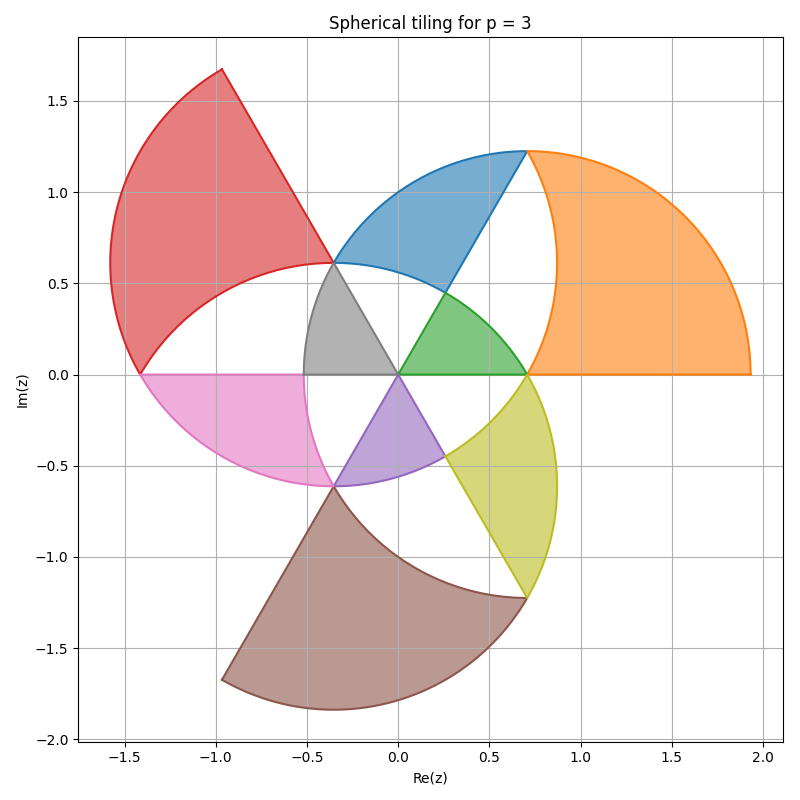
\includegraphics[width=0.45\linewidth]{images/tiling_3.png}
    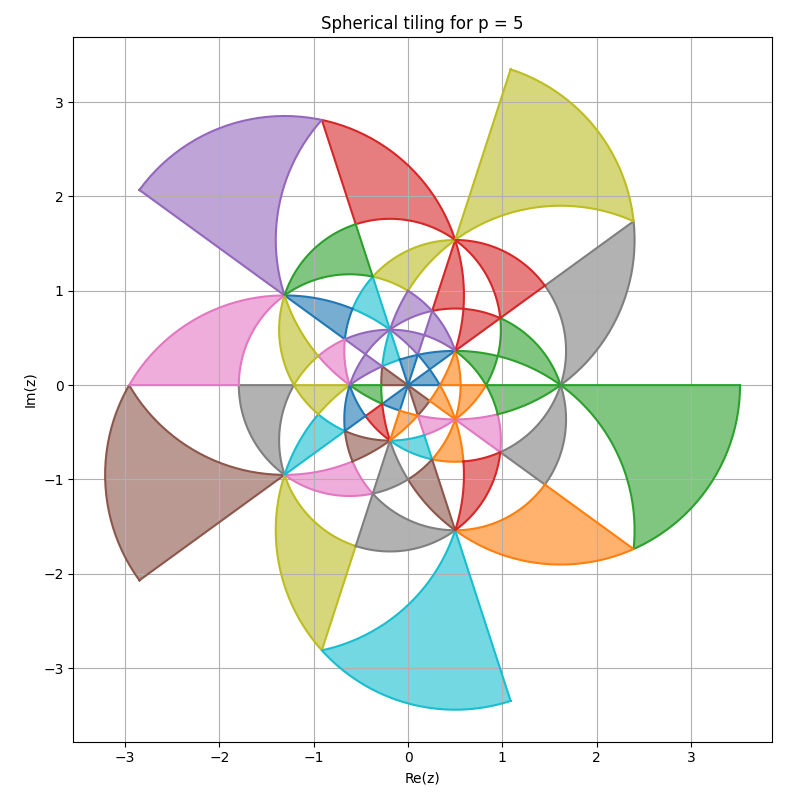
\includegraphics[width=0.45\linewidth]{images/tiling_5.png}
    \caption{Spherical tessellations with large triangles omitted.}
\end{figure}

Furthermore, no two admissible triangles can overlap. Suppose the interiors of two distinct generated triangles overlap, 
\[ \Delta_g^\circ \cap \Delta_h^\circ \neq \emptyset, \]
where \(\Delta_g = S_g(\Delta_0)\), \(\Delta_h = S_h(\Delta_0)\), and \(S_g \neq S_h\). Let \(z\) be a point in the interior intersection. Then \(z = S_g(w_g)\) and \(z = S_h(w_h)\) for some \(w_g, w_h \in \Delta_0^\circ\). Applying the inverse transformation \(S_h^{-1}\), we get \(S_h^{-1}(z) = w_h\). Substituting \(z = S_g(w_g)\), we have 
\[S_h^{-1}(S_g(w_g)) = w_h.\]
Let \(S_k = S_h^{-1} \circ S_g \neq e\) so \(S_k(w_g) = w_h\). This is a contradiction, as a defining property of a fundamental domain for a discrete group action is that distinct points in its interior belong to different orbits.

\begin{figure}
    \centering
    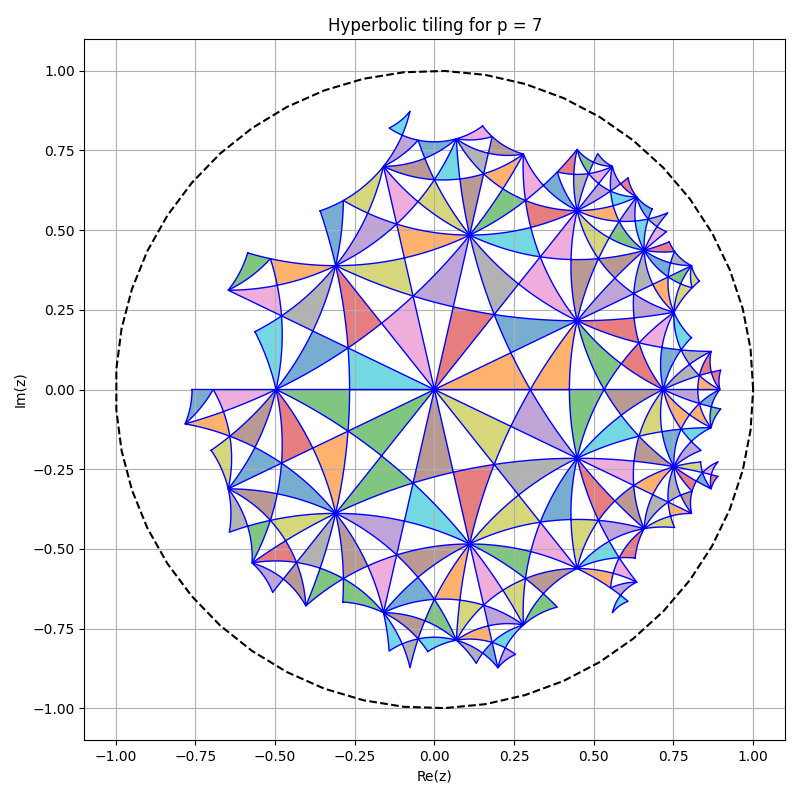
\includegraphics[width=1.0\linewidth]{images/tiling_7.png}
    \caption{Hyperbolic tessellation for \(n = 7\).}
\end{figure}

The cases \(p = 3\) and \(p = 5\) correspond to the symmetry groups of the tetrahedron and icosahedron respectively. We have the isomorphisms \(\mathrm{PSL}(2,3)\sim A_4\), \(\mathrm{PSL}(2,5)\sim A_5\)

\section{Visualisations in Python}

Throughout this project and previous project, we have seem the Matplotlib library in Python is useful for visualisation of two-dimensional information, such as scatter plots, line plots and filled shapes. 

To view three-dimensional visualisations, we can import the mplot3d toolkit which is particularly helpful for computational geometry. In particular, we can plot parametrisations of curves or surfaces given an immersion; level curve or sets of a submersion; and entire \(3\)D-graphs of functions. 

\begin{minted}[autogobble]{python}
    fig = plt.figure(figsize = (8,8))
    ax = plt.axes(projection='3d')
    ax.grid()
    t = np.arange(0, 10*np.pi, np.pi/50)
    x = np.sin(t)
    y = np.cos(t)
    
    ax.plot3D(x, y, t)
    ax.set_title('3D Parametric Plot')
    
    ax.set_xlabel('x', labelpad=20)
    ax.set_ylabel('y', labelpad=20)
    ax.set_zlabel('t', labelpad=20)
    
    plt.show()
\end{minted}

\begin{minted}[autogobble]{python}
    fig = plt.figure(figsize = (12,10))
    ax = plt.axes(projection='3d')
    
    x = np.arange(-5, 5.1, 0.2)
    y = np.arange(-5, 5.1, 0.2)
    
    X, Y = np.meshgrid(x, y)
    Z = np.sin(X)*np.cos(Y)
    
    surf = ax.plot_surface(X, Y, Z, cmap = plt.cm.cividis)

    ax.set_xlabel('x', labelpad=20)
    ax.set_ylabel('y', labelpad=20)
    ax.set_zlabel('z', labelpad=20)
    
    fig.colorbar(surf, shrink=0.5, aspect=8)
    
    plt.show()
\end{minted}


More advanced techniques include working with maps or creating animations and movies.

\end{document}
